\documentclass[10pt,a4paper]{book}
%----------------------------------------------------------
% This is a sample document for the standard LaTeX Book Class
% Class options
%       --  Body text point size:
%                        10pt (default), 11pt, 12pt
%       --  Paper size:  letterpaper (8.5x11 inch, default)
%                        a4paper, a5paper, b5paper,
%                        legalpaper, executivepaper
%       --  Orientation (portrait is the default):
%                        landscape
%       --  Printside:   oneside, twoside (default)
%       --  Quality:     final(default), draft
%       --  Title page:  titlepage, notitlepage
%       --  Columns:     onecolumn (default), twocolumn
%       --  Start chapter on left:
%                        openright(no, default), openany
%       --  Equation numbering (equation numbers on right is the default):
%                        leqno
%       --  Displayed equations (centered is the default):
%                        fleqn (flush left)
%       --  Open bibliography style (closed bibliography is the default):
%                        openbib
% For instance the command
%          \documentclass[a4paper,12pt,reqno]{book}
% ensures that the paper size is a4, fonts are typeset at the size 12p
% and the equation numbers are on the right side.


\usepackage[left=2.5cm, right=2cm, top=2cm, bottom=2cm]{geometry}
\usepackage[latin1]{inputenc}
\usepackage[T1]{fontenc}
\usepackage{pdflscape}
\usepackage[colorlinks,pdfpagelabels,pdfstartview = FitH,bookmarksopen = true,bookmarksnumbered = true,linkcolor = black,plainpages = false,hypertexnames = false,citecolor = black] {hyperref}

\usepackage{amsmath}
\usepackage{amsfonts}
\usepackage{amssymb}
\usepackage{amsthm}
\usepackage{upgreek}


\usepackage{graphicx}
\usepackage{color}
\usepackage{tikz}
	\usetikzlibrary{shapes,arrows}
\usepackage{dirtree}

\usepackage{tabularx}
%\usepackage{ltablex}
\usepackage{multicol}

\usepackage{listings}
\usepackage{blindtext}

\usepackage{float}
\usepackage[section]{placeins}
\usepackage{wrapfig}
\usepackage{caption}
\usepackage{subcaption}


%\usepackage[printonlyused,withpage]{acronym}
\usepackage{makeidx}
\usepackage{cite}
\usepackage[acronym,shortcuts,toc]{glossaries}

%%%%%%%%%%% Personal commands %%%%%%%%%%%%%%%%%

\newcommand{\software}{{\scshape TOM }}
\newcommand{\matlab}{{\scshape MATLAB }}
\newcommand{\omen}{{\scshape OMEN }}

\theoremstyle{remark}
\newtheorem*{REMARK}{Remark}
\newtheorem*{EXAMPLE}{Example}

%%%%%%%%%%%%%%%%%%%%%%%%%%%%%%%%%%%%%%%%%%%%%%%


\lstset{language=Matlab}
\setlength\parindent{0pt}

\makeindex
\makeglossaries

\definecolor{mygreen}{rgb}{0,0.6,0}
\definecolor{mygray}{rgb}{0.5,0.5,0.5}
\definecolor{mymauve}{rgb}{0.58,0,0.82}

\lstset{ %
  backgroundcolor=\color{white},   % choose the background color; you must add \usepackage{color} or \usepackage{xcolor}
%  basicstyle=\footnotesize,        % the size of the fonts that are used for the code
  breakatwhitespace=false,         % sets if automatic breaks should only happen at whitespace
  breaklines=true,                 % sets automatic line breaking
  captionpos=b,                    % sets the caption-position to bottom
  commentstyle=\color{mygreen},    % comment style
  deletekeywords={...},            % if you want to delete keywords from the given language
  escapeinside={\%*}{*)},          % if you want to add LaTeX within your code
  extendedchars=true,              % lets you use non-ASCII characters; for 8-bits encodings only, does not work with UTF-8
  frame=single,                    % adds a frame around the code
  keepspaces=true,                 % keeps spaces in text, useful for keeping indentation of code (possibly needs columns=flexible)
  keywordstyle=\color{blue},       % keyword style
  language=Matlab,                 % the language of the code
  morekeywords={*,...},            % if you want to add more keywords to the set
  numbers=left,                    % where to put the line-numbers; possible values are (none, left, right)
  numbersep=5pt,                   % how far the line-numbers are from the code
  numberstyle=\tiny\color{mygray}, % the style that is used for the line-numbers
  rulecolor=\color{black},         % if not set, the frame-color may be changed on line-breaks within not-black text (e.g. comments (green here))
  showspaces=false,                % show spaces everywhere adding particular underscores; it overrides 'showstringspaces'
  showstringspaces=false,          % underline spaces within strings only
  showtabs=false,                  % show tabs within strings adding particular underscores
  stepnumber=2,                    % the step between two line-numbers. If it's 1, each line will be numbered
  stringstyle=\color{mymauve},     % string literal style
  tabsize=2,                       % sets default tabsize to 2 spaces
  title=\lstname                   % show the filename of files included with \lstinputlisting; also try caption instead of title
}
%\usepackage{ETH light}
%----------------------------------------------------------

%\includeonly{Chapters/ProcessingQDots}

\begin{document}

\frontmatter
\cleardoublepage\pdfbookmark{\titlepage}{Titlepage}
\newcommand{\trtitle}{Simulation of Quantum Dots}
\newcommand{\trtype}{Group project}
\newcommand{\trprofone}{Prof. Vanessa Wood}
\newcommand{\trproftwo}{Prof. Mathieu Luisier}
\newcommand{\trresearchgroup}{Laboratory for Nanoelectronics}
\newcommand{\trinstitute}{Integrated Systems Laboratory}
\newcommand{\trdepartment}{Department of Information Technology \& Electrical Engineering}
\newcommand{\truni}{ETH Zurich}
\newcommand{\trdate}{\today}

\thispagestyle{empty}


\includegraphics[scale=0.8]{Fig/eth_logo_black.pdf}

\rule{\textwidth}{0.4pt}

\vspace{2.5cm}
\begin{center}
  \textbf{\LARGE \trtitle}
\end{center}
\vspace{2cm}

\begin{center}
  \textbf{\trtype}	\\
  \trresearchgroup	\\
  \trprofone				\\
  \trinstitute			\\
  \trdepartment			\\
  \truni						\\[0.5cm]
  Handed in by			\\
  \textbf{Christian Funck \& Matthias Dittberner}	\\[0.5cm]
  Date							\\
  \trdate						\\
\end{center}

\vspace{1cm}

\begin{center}
	\begin{tabular}{ll}
		Supervisor: & \trprofone	\\
								& \trproftwo	\\
	\end{tabular}
\end{center}

\vfill

%\begin{tabularx}{\textwidth}{lr}
\begin{tabular*}{\textwidth}{@{\extracolsep{\fill} } lr}
%\begin{tabular}{@{}p{0.5\textwidth}>{\raggedright\arraybackslash}{p{0.5\textwidth}}}
	Christian Funck					&	Matthias Dittberner				\\
	Plattenstrasse 71				&	Luegislandstrasse 269			\\
	8032 Zurich							&	8051 Zurich								\\
	09-920-177							& 09-913-450								\\
	cfunck@student.ethz.ch	&	mdittber@student.ethz.ch	\\
\end{tabular*}

\rule{\textwidth}{0.4pt}

\cleardoublepage\pdfbookmark{\contentsname}{toc}		% Add Table of Contents to the PDF bookmarks
\tableofcontents
\newpage


%\chapter{Preface}

%\chapter{Introduction}



\mainmatter

\chapter{The Quantum Dot} \label{sec:QuantumDot} \index{Quantum Dot}

	Quantum dots are atomic structures (usually spherical) that have a size of about 1-10nm in diameter. They are often referred to as \glspl{NC}, though this
	term is more general and includes also other shapes and morphologies, which might extend to several $\mu$m, such as rods, wires etc.
	Figure \ref{fig:QDshapes} gives some examples of possible shapes and morphologies, that are possible with nowadays technologies.
	
	\glspl{QD} are possible with various materials such as metals, semiconductors and compounds. According to their size and material,
	a \glspl{QD} can contain just a few or millions of atoms. A 10nm cube of GaAs contains for example 40,000 atoms \cite{SalehTeich}.
	
	The properties of \glspl{QD} are strongly dependent on their size. Figure \ref{fig:QDTheory} illustrates this effect for a semiconductor \gls{QD}.
	Under ultraviolet excitation, the \glspl{QD} emit light according to their size and therefore band gap.
	
	\begin{figure}[htbp]
		\begin{minipage}[t]{0.49\textwidth}
			\centering
			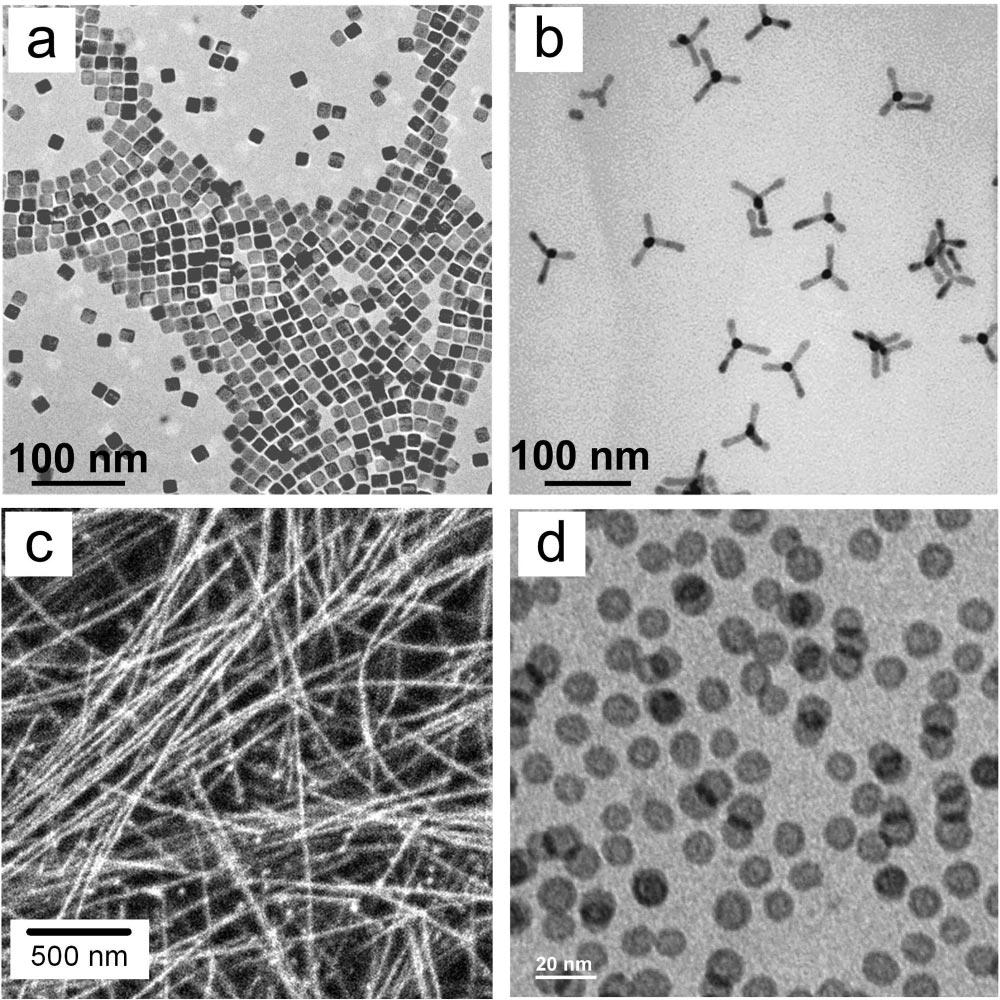
\includegraphics[width=\textwidth]{Fig/QDshapes.jpg}
			\caption{Examples of inorganic nanomaterials with different
							 shapes and morphologies synthesized by colloidal chemistry:
							 (a) PbSe cubes; (b) CdTe tetrapods; (c) PbSe nanowires and
							 (d) hollow iron oxide nanoparticles.
							 {\scshape Source:} \cite[p.394]{Talapin}}
			\label{fig:QDshapes}
		\end{minipage}
		\hfill
		\begin{minipage}[t]{0.49\textwidth}
			\centering
			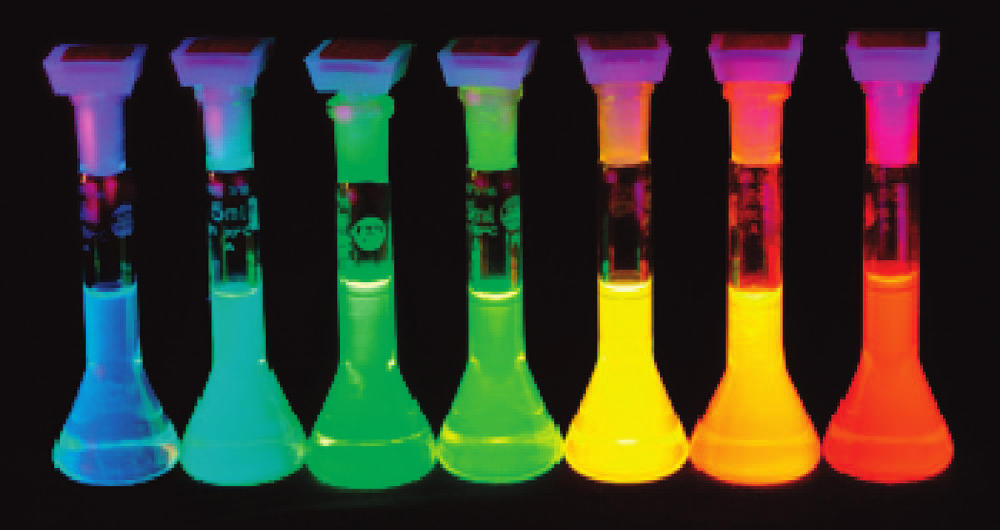
\includegraphics[width=\textwidth]{Fig/QDcolor.jpg}
			\caption{This photograph shows the size-dependent \gls{PL} of the quantum dots. The particles with the smallest ($\sim$1.7nm)
							 CdSe cores emit blue and those with the largest cores ($\sim$5nm) emit red.
							 {\scshape Source:} \cite[p.393]{Talapin}}
			\label{fig:QDcolor}
		\end{minipage}
	\end{figure}			

	\paragraph{Basic physics of the Quantum Dot}
		For bulk materials the band gap \index{Band gap} is a fixed parameter, that specifies the type of material. But when a particle gets smaller and reaches
		a size of about 10nm this will not be the case anymore. The band gap is than depending on the size of this particle (\glspl{NC}). As
		the mobility of the charge carriers (electrons, holes) is very limited in all three dimensions in the quantum dot, the energy levels
		are not continuous, but instead discrete.
		This phenomenon is called the {\it quantum size effect}.
		
		The band gap \index{Band gap} of a spherical \gls{QD} of radius $R$ is then approximately:
		\begin{equation}
			E_{g} \approx E_{g,0} + \frac{\hbar^2 \pi^2}{2 m_{eh} R^2}
			\label{eq:Bandgap}
		\end{equation}
		where $E_{g,0}$ denotes the band gap of the bulk material and $m_{eh}$ is obtained through the effective masses of electrons and holes $m_{e,p}$:
		\begin{equation}
			m_{eh} = \frac{m_e m_h}{m_e + m_h}
			\label{eq:QuantumBox}
		\end{equation}
		
		\begin{figure}[htbp]
			\centering
			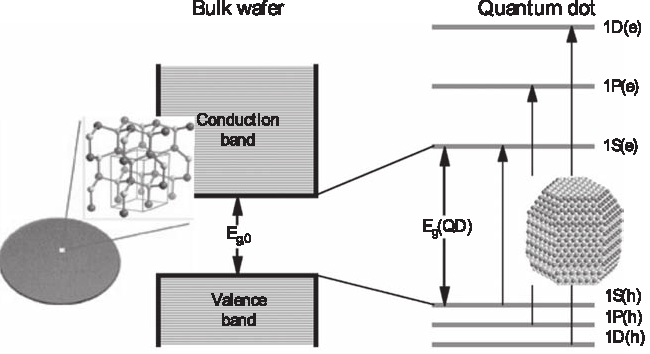
\includegraphics[width=0.4\textwidth]{Fig/QDTheory.pdf}
			\caption{The left illustration shows the band structure of a bulk semiconductor with energy band gap $E_{g,0}$,
							 whereas the the right one illustrates the discrete energy levels of a \gls{QD} and its energy gap $E_{g}(QD)$.
							 {\scshape Source:} \cite[p.3]{Klimov}}
			\label{fig:QDTheory}
		\end{figure}
		
		
		We will see later in chapter \ref{sec:BandGapAnalysis} that the \gls{QD} absorption spectrum \index{Absorption spectrum} as shown in figure \ref{fig:QDTheory}(c) is not really discrete; as it is
		not possible to fabricate \glspl{QD} that are perfectly equal in size, this results in a broadening of the spectrum.
		The energy gap increases for decreasing \gls{QD} sizes, because more energy is required to confine the electron to a smaller volume.
		This is caused by Heisenberg's uncertainty principle \index{Heisenberg uncertainty principle}, which says, that if we want to locate a particle of effective mass $m$ (for example an electron),
		on an x-axis within an interval	$\Delta x$, we can only make an uncertain prediction of its impulse. If the spatial region gets smaller, the uncertainty
		of the impulse will	increase.
		\begin{equation}
			\Delta p_{x} \sim \frac{\hbar}{\Delta x}
		\end{equation}
		This adds to the kinetic energy of the free particle, which is called the confinement \index{Confinement} energy \index{Confinement!Energy}, that has an significant impact, if it gets bigger
		than the thermal energy of the particle.
		\begin{equation}
			E_{confinement} = \frac{(\Delta p_{x})^2}{2 m} \sim \frac{\hbar^2}{2 m (\Delta x)^2} > \frac{1}{2} k_{B} T
		\end{equation}
		From this we can conclude, that the quantum size effect is relevant if
		\begin{equation}
			\Delta x < \sqrt{\frac{\hbar^2}{m k_{B} T}}
		\end{equation}
		Table \ref{tbl:ConfinedStr} shows 4 possible confinement structures\index{Confinement!Structure}, which are illustrated in Figure \ref{fig:ConfinedStr} with their
		characteristic energy levels \index{Energy level} in	the conduction band.

		\begin{figure}[htbp]		
		\centering
		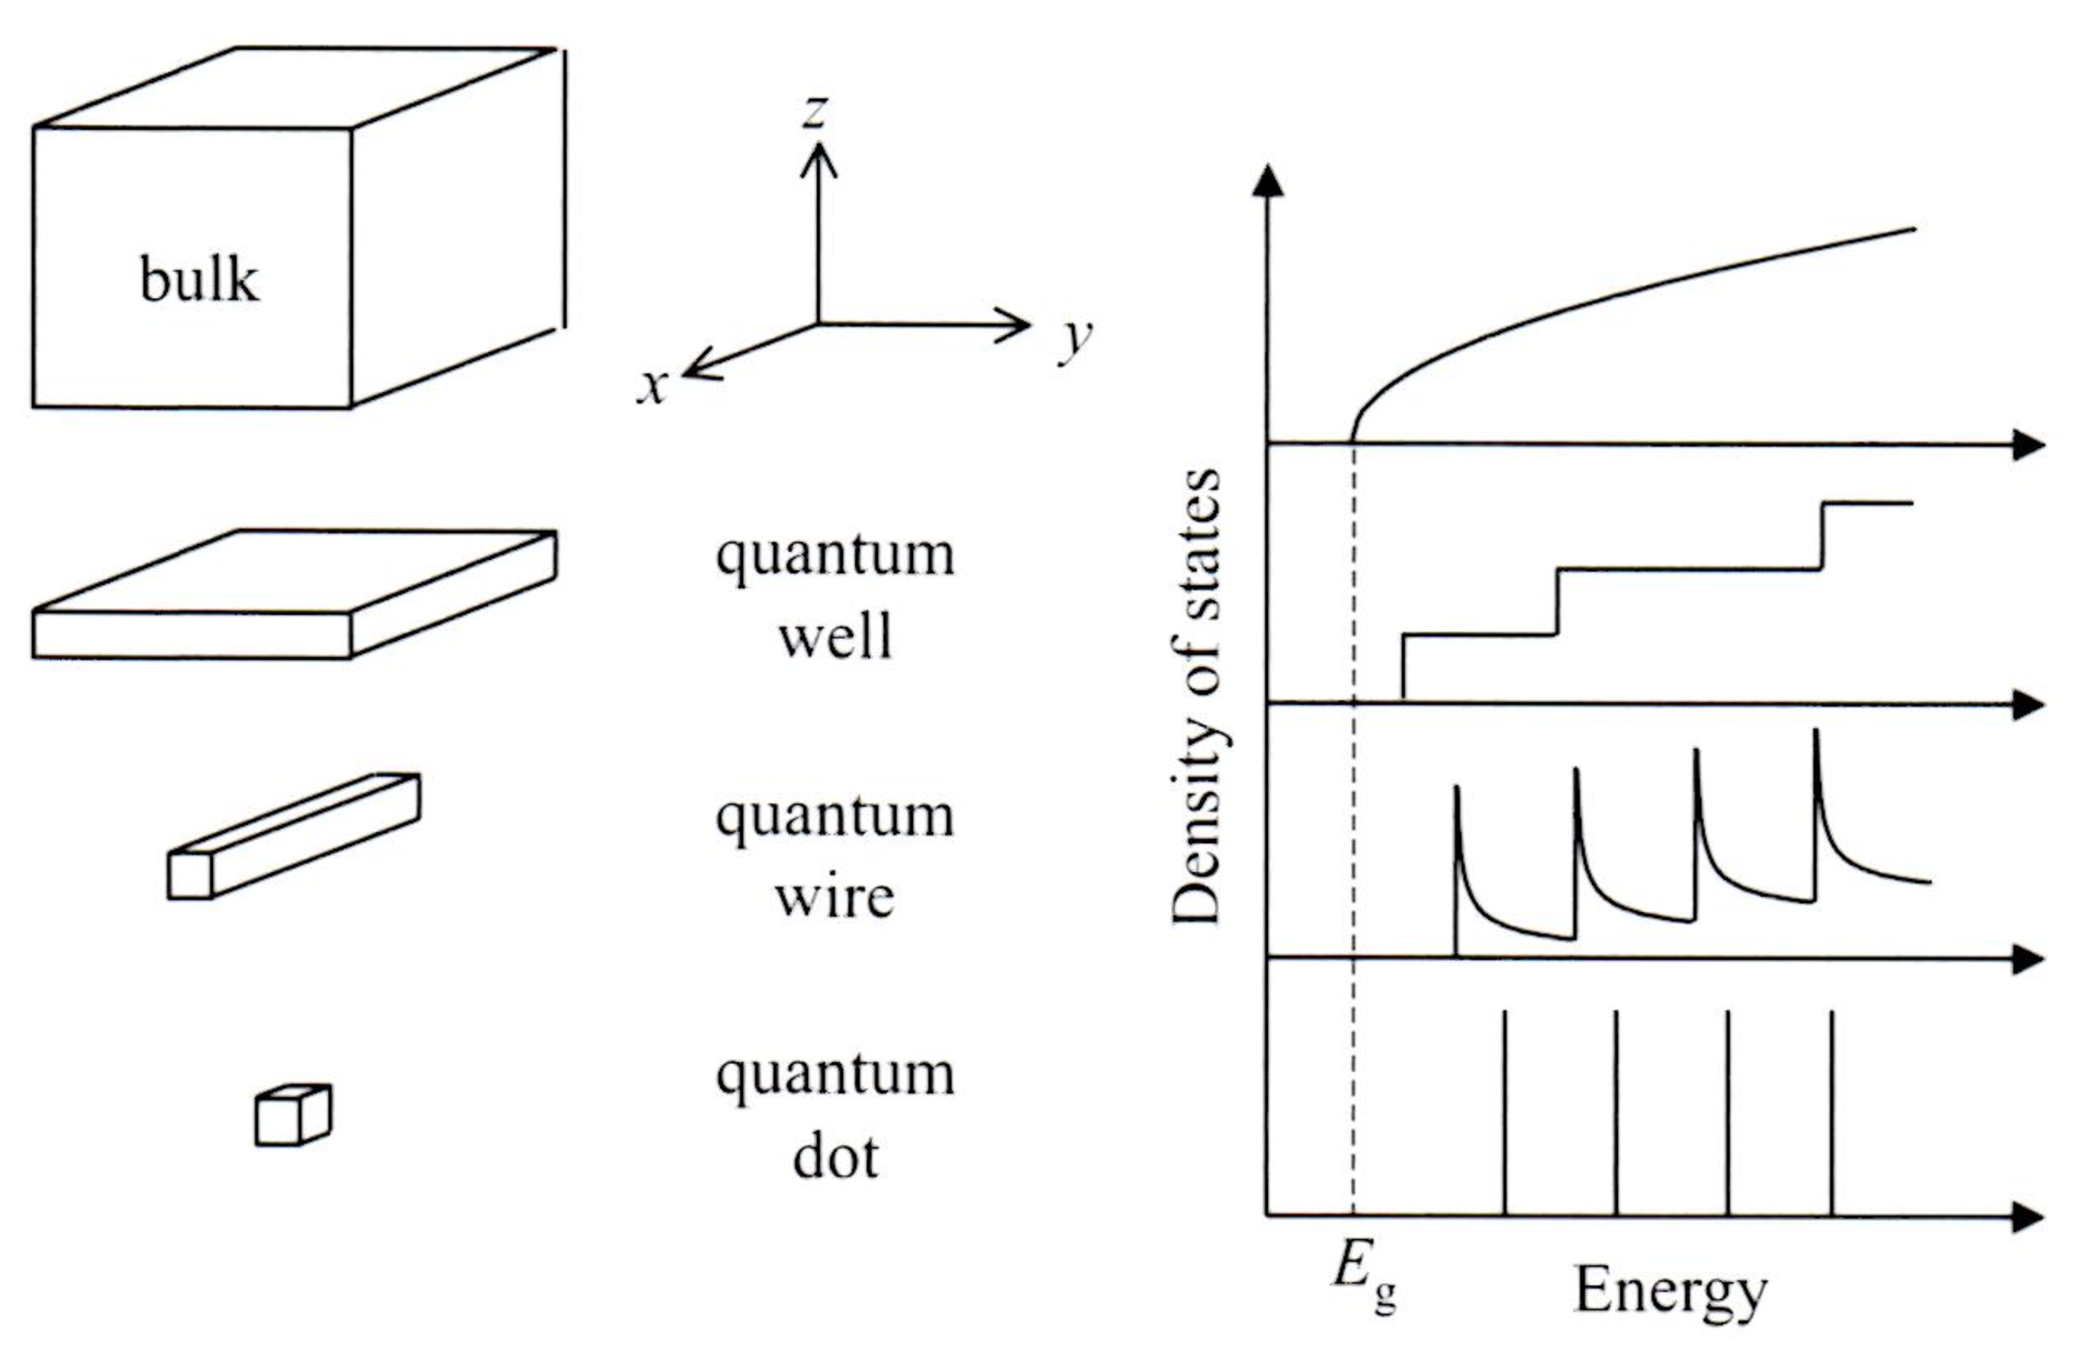
\includegraphics[width=0.5\textwidth]{Fig/ConfinedStructures.pdf}
		\caption{Schematic representation of quantum wells, wires and dots (left).
						 The generic shape of the density of states function for electrons in the
						 conduction band of a semiconductor with band gap $E_{g}$ is shown for each
						 type of the structure (right).
						 {\scshape Source:} \cite[p.143]{Fox}}
		\label{fig:ConfinedStr}
	\end{figure}
		
		\begin{table}[htbp]
		\centering
			\begin{tabular}{lccc}
				Structure											&	Quantum				&	\# of free		&	Electron						\\
																			&	confinement		&	dimensions		&	density of states		\\
				\hline
				Bulk													&	none					&	3							&	$\propto E^{1/2}$		\\
				Quantum well/superlattice			&	1-D						&	2							&	$\propto E^{0}$			\\
				Quantum wire									&	2-D						&	1							&	$\propto E^{-1/2}$	\\
				Quantum dot/box								&	3-D						&	0							&	discrete						\\
			\end{tabular}
			\caption{Number of degrees of freedom tabulated against the dimensionality of the quantum confinement.
							 The final column shows the functional form of the density of states for free electrons.
							 {\scshape Source:} \cite[p.142]{Fox}}
			\label{tbl:ConfinedStr}
		\end{table}
	
	\paragraph{Fabrication techniques of \gls{QD}}
	
		A lot of different ways to make \glspl{QD} have been developed. Research efforts are made to create
		more efficient \glspl{QD} and new shapes and morphologies. As \glspl{QD} are more and more interesting for various commercial applications,
		low costs play an important factor. The colloidal chemistry has made a major contribution, as it offers low energy
		synthesis of \glspl{NC}/\glspl{QD} using very simple and affordable laboratory equipment.		
		In the next chapter we will briefly discuss the mentioned technique, by giving a short overview
		that avoids the use of chemical terms as much as possible, rather than a detailed disquisition, as this is a research field on its own.
		
		Some other methods are listed below.
	
		\begin{tabularx}{\textwidth}{Xl}
			{\bf Physical methods}														&	{\bf Characterization}										\\
			Molecular-beam-epitaxy (MBE)											& High-energy-input, expensive apparatus,
																													used	for \glspl{QD}											\\
			Metalorganic-chemical-vapor-decomposition (MOCVD)	&	High-energy-input, used for \glspl{QD}		\\
			Vapor-liquid-solid (VLS)													&	High-energy-input, used for quantum wires	\\
			Electron-beam lithography													&			\\
																												&			\\
			{\bf Chemical methods}														&	{\bf Characterization}										\\
			Colloidal chemical synthesis of crystalline
			semiconductor nanoparticles												& Low-energy-input, wet chemistry,
																													used for various structures								\\
		\end{tabularx}
	
		
		
	\paragraph{Applications}
		
		In biology and chemistry \glspl{QD} are used as spectral tags that are attached to molecules, making their position visible for identification
		under optical illumination. In the past, one used organic dyes, but compared to \glspl{QD} the sharpness of emission lines is not as good.
		
		In electronics, \glspl{QD} are used to increase the efficiency of lasers \cite{SemiconductorCD}, everyday light sources and solar cells.
		Furthermore they are used	in broadband \gls{LED}, memory elements, flexible displays, photodetectors.
		
		We have to add that a lot of these applications are still developed in research institutions and are not yet available for commercial use.
		
		Although the applications seem impressive and will probably motivate new technologies, there are reasonable concerns about these nanoscale
		particles. Some of the materials are toxic and through the small sizes it is unclear what might happen if the particles end up in living
		organisms or generally speaking, into the the environment.
		For more interested readers, we recommend the following paper for further reading: \citeauthor{Hardman} \citetitle{Hardman} \cite{Hardman}.

\chapter{Simulations}

	\section{Technical Aspects}
		Our simulation results are based on OMEN which uses tight binding parameters by Lent et. al \cite{Lent1986}

\chapter{Conclusion / Summary}
%%\acl{CQD}
%%
%	\begin{appendix}
%		\chapter{Abbreviations}
%%			
%%
%			\begin{acronym}[ARB]
%%				%\setlength{\itemsep}{-\parsep}
%				\acro{CQD}{Colloidal Quantum Dot}
%				\acro{YTM}{Yield to Maturity, Endf�lligkeitsrendite}
%			\end{acronym}
%	\end{appendix}
	

		
	%%%%%%%%%%%%%%%%%%%%%%%%%%%% Glossary - Begin %%%%%%%%%%%%%%%%%%%%%%%%%%%%%%
	
	\glossary{name={Colloidal Quantum Dots}, description={The Fermi level also known as the Fermi Energy
						is the Energy at which the probability of finding an Electron/Hole is equal to 50\%. \newline
						At equilibrium the Fermi Level must be flat throughout the entire structure.}}
		
	
	%%%%%%%%%%%%%%%%%%%%%%%%%%%  Glossary - End %%%%%%%%%%%%%%%%%%%%%%%%%%%%%%%%

	\clearpage
	\printglossary
	
	\clearpage
	\phantomsection
	\addcontentsline{toc}{chapter}{\indexname}
	\printindex
	
	\clearpage
	\phantomsection
	\addcontentsline{toc}{chapter}{References}
		\nocite{Klimov}
		\nocite{DLTS_paper}
		\nocite{Hines2003}
		\nocite{Ip2012}
		\nocite{Tang2011}
		\nocite{Cademartiri2006}
		\nocite{Efros2000}
		\nocite{Lent1986}
		\nocite{OMENmanual}
	\bibliography{Bibliography}
	\bibliographystyle{plain}
	
	\clearpage
	\phantomsection
	\addcontentsline{toc}{chapter}{List of Tables}
	\listoftables
	
	
	\backmatter
	
	\chapter{Declaration of Originality}

	We hereby declare that the written work we have submitted entitled
	
	\vspace{0.5cm}
	
	{\bf \hspace{0.5cm} \trtitle}
	
	\vspace{0.5cm}
	
	is original work which we alone have authored and which is written in our own words.
	
	\vspace{1cm}
	
	\hspace{0.5cm} 
	\begin{tabular}{lll}
		{\bf Authors}				&											&									\\
		{\sc Last name}			&	{\sc First name}		&									\\
		Dittberner					& Matthias						&									\\
		Funck								&	Christian						&									\\
		\\
		\\
		{\bf Supervisors}		&											&									\\
		{\sc Last name}			&	{\sc First name}		& {\sc Degree}		\\
		Luisier							&	Mathieu							& Professor				\\
		Wood								&	Vanessa							& Professor
	\end{tabular}
	
	\vspace{1cm}
	
	With the signature we declare that we have been informed regarding normal academic
	citation rules and that we have read and understood the information on {\it Citation etiquette}
	(\url{http://www.ethz.ch/students/exams/plagiarism_s_en.pdf}). The citation conventions
	usual to the discipline in question	here have been respected.
	The above written work may be tested electronically for plagiarism.
	\footnote{Based on the official Declaration of ETH Zurich:
	\url{http://www.ethz.ch/faculty/exams/plagiarism/confirmation_en.pdf}}
	
	\vspace{3.5cm}
	
	\begin{tabular*}{\textwidth}{@{\extracolsep{\fill}} lclcrcr}
		Place and date & \hspace{0.5cm} & Christian Funck	& \hspace{2.5cm} &	Place and date	& \hspace{0.5cm} & Matthias Dittberner	
	\end{tabular*}

	
\end{document}